% !TEX encoding = UTF-8
% !TEX TS-program = pdflatex
% !TEX root = ../tesi.tex

%**************************************************************
\chapter{Modello Bradley-Terry e i numeri di gol }
\label{cap:risFin}
%**************************************************************
\intro{In questo capitolo si illustreranno i risultati ottenuti con il modello Bradley-Terry (\ref{for:4.9}) con una variabile risposta a cinque categorie legate al numero di gol segnati dalle squadre durante le partite.
}
%**************************************************************
\section{Premessa}
Nel Capitolo \ref{cap:risultatiDM} si era sottolineato che i risultati ottenuti non tenevano in considerazione le variabili esplicative gol fatti \textsf{GF} e gol subiti \textsf{GA}, a causa della non convergenza del modello. Per poter utilizzare queste due variabili esplicative, su ispirazione del lavoro di ricerca di \textcite{schauberger2017}, si è deciso di cambiare il numero di categorie della variabile risposta \emph{Y} ovvero, di utilizzare cinque categoria al posto di tre, in base al numero di gol segnati e subiti, nello specifico:
\begin{equation}
	Res =
	\begin{cases}
		1 & \text{se la squadra in casa batte la squadra ospite con due gol di scarto,}\\
		2 & \text{se la squadra in casa batte la squadra ospite con un gol di scarto,}\\
		3 & \text{se la partita termina con un pareggio,}\\
		4 & \text{se la squadra ospite batte la squadra in casa con un gol di scarto. }\\
		5 & \text{se la squadra ospite batte la squadra in casa con due gol di scarto.}
	\end{cases}       
\end{equation}

\section{Modello Bradley-Terry con Y=5 e Lasso}
I risultati ottenuti dal modello (\ref{for:4.9}) con \emph{Y = 5} sono presentanti nella Figura \ref{tab:BTCL5} e nella Tabella \ref{}. Nella Figura \ref{tab:BTCL5} si può notare che le stime dall'abilità delle squadre è molto simile a quelle riportate nella Figura \ref{tab:BTCL}. Infatti, nelle prime e nelle ultime quattro posizioni la stima e il piazzamento rimangono invariati. Cambiano le stime di Atalanta, Lazio e Roma infatti, abbiamo che: l'Atalanta aumenta la propria stima e quindi viene ancora più sovrastimata, mentre per Lazio e Roma l'abilità stimata cala. Anche Fiorentina e Hellas Verona hanno un aumento dell'abilità stimata, anche se l'Hellas Verona viene sovrastimata rispetto alla Fiorentina. Infine, anche l'Empoli aumenta la propria abilità stimata tanto da essere stimato più forte del Bologna e quindi sovrastimato.

\begin{sidewaysfigure} 
	\centering
	\begin{center}
		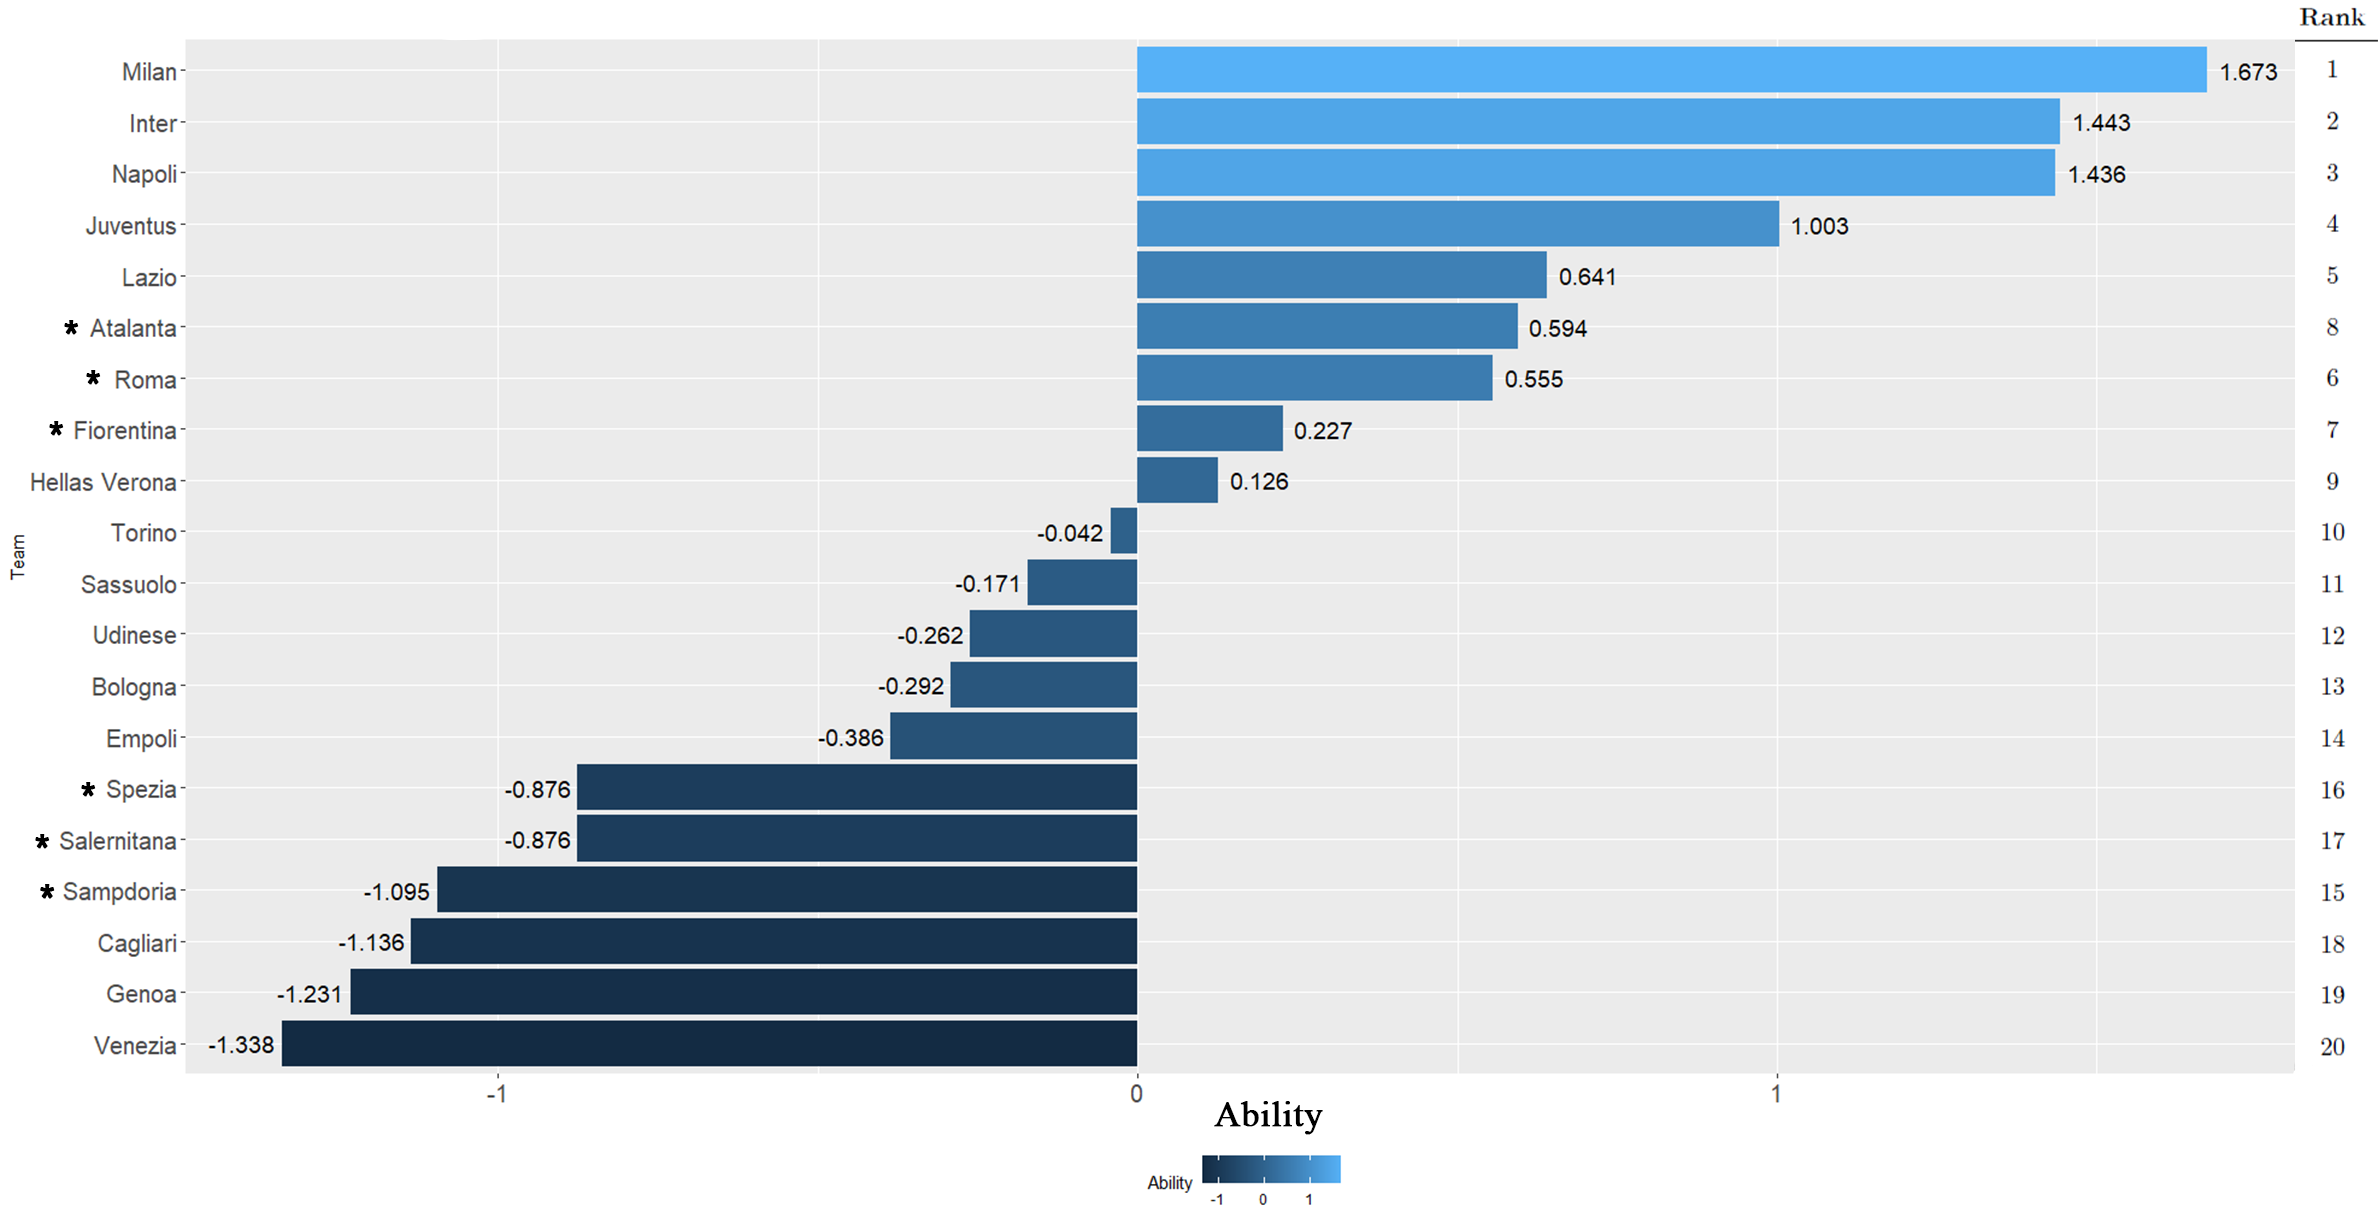
\includegraphics[height=13cm, width=23cm]{rank3.png}
		\caption{Barplot che indica per ogni squadra l'abilità stimata dal modello (\ref{for:4.9}) con Y = 5. Viene indicato con un asterisco le squadre con un piazzamento stimato diverso da quello reale anche esso riportato a destra del grafico.} \label{tab:BTCL5} 
	\end{center}
\end{sidewaysfigure}